\documentclass[a4paper,12pt]{article}
\usepackage[utf8]{inputenc}
\usepackage{graphicx}
\usepackage{graphics}
\usepackage{hyperref}
\usepackage{geometry}
\usepackage{caption}
\usepackage{pdflscape}

\graphicspath{ {build/} } 
\geometry{left=2cm, right=2cm, top=2cm, bottom=2cm}

\begin{document}

\begin{titlepage}
    \begin{center}
        \vspace*{3cm}
        
        {\Huge \textbf{Laboratorio 1 - Grupo 7}}\\[1cm]
        {\LARGE Panel solar automático:\\ [0.5cm]Acta de constitución de Proyecto}\\[2cm]
        
        \vfill
        
        {\Large \textbf{Integrantes }}\\[.5cm]
        \large
        \begin{tabular}{c c}
            Gartner, Francisco Nehuen & 69864/6 \\
            Marchesotti, Guido Daniel & 69923/9 \\
            Rosa, Fausto Pablo & 69843/1 \\
        \end{tabular}
        
        \vspace{1cm}
        
        \begin{figure}[b]
            \centering
            
\includegraphics[width=1\linewidth]{LOGOSFI-UNLP-color-01.png}
        \end{figure}
        
        %%{\large \today}
    \end{center}
\end{titlepage}

%%\newpage
%%\tableofcontents
%%\newpage

\section{Visión general del proyecto}
%%\hfill{ }\\ {\large \textbf{Visión general del proyecto:}}\\


El siguiente documento constituye el acta de planificación del proyecto "Panel solar automático", cuyo propósito consistiría en desarrollar un sistema automatizado de seguimiento solar. Esta iniciativa tendría como objetivo optimizar la captación de energía por parte de un panel solar fotovoltaico, mediante la modificación dinámica de su orientación utilizando un sistema de control de 2 ejes. Tal mecanismo permitiría maximizar la potencia instantánea, esperando superar el rendimiento de los paneles con orientación fija y mejorando así la eficiencia energética del sistema en su conjunto.\\

Adicionalmente, se planearía la implementación de un sistema de monitoreo que almacenaría y transmitiría los datos recolectados sobre la potencia generada. Estos datos serían enviados a través de una conexión inalámbrica hacia una aplicación móvil, en la cual el usuario podría consultar información en una interfaz gráfica intuitiva. Esta aplicación permitiría visualizar los registros históricos de las mediciones, facilitando el análisis y la trazabilidad del desempeño energético.\\

\begin{figure}[h!]
    \centering
    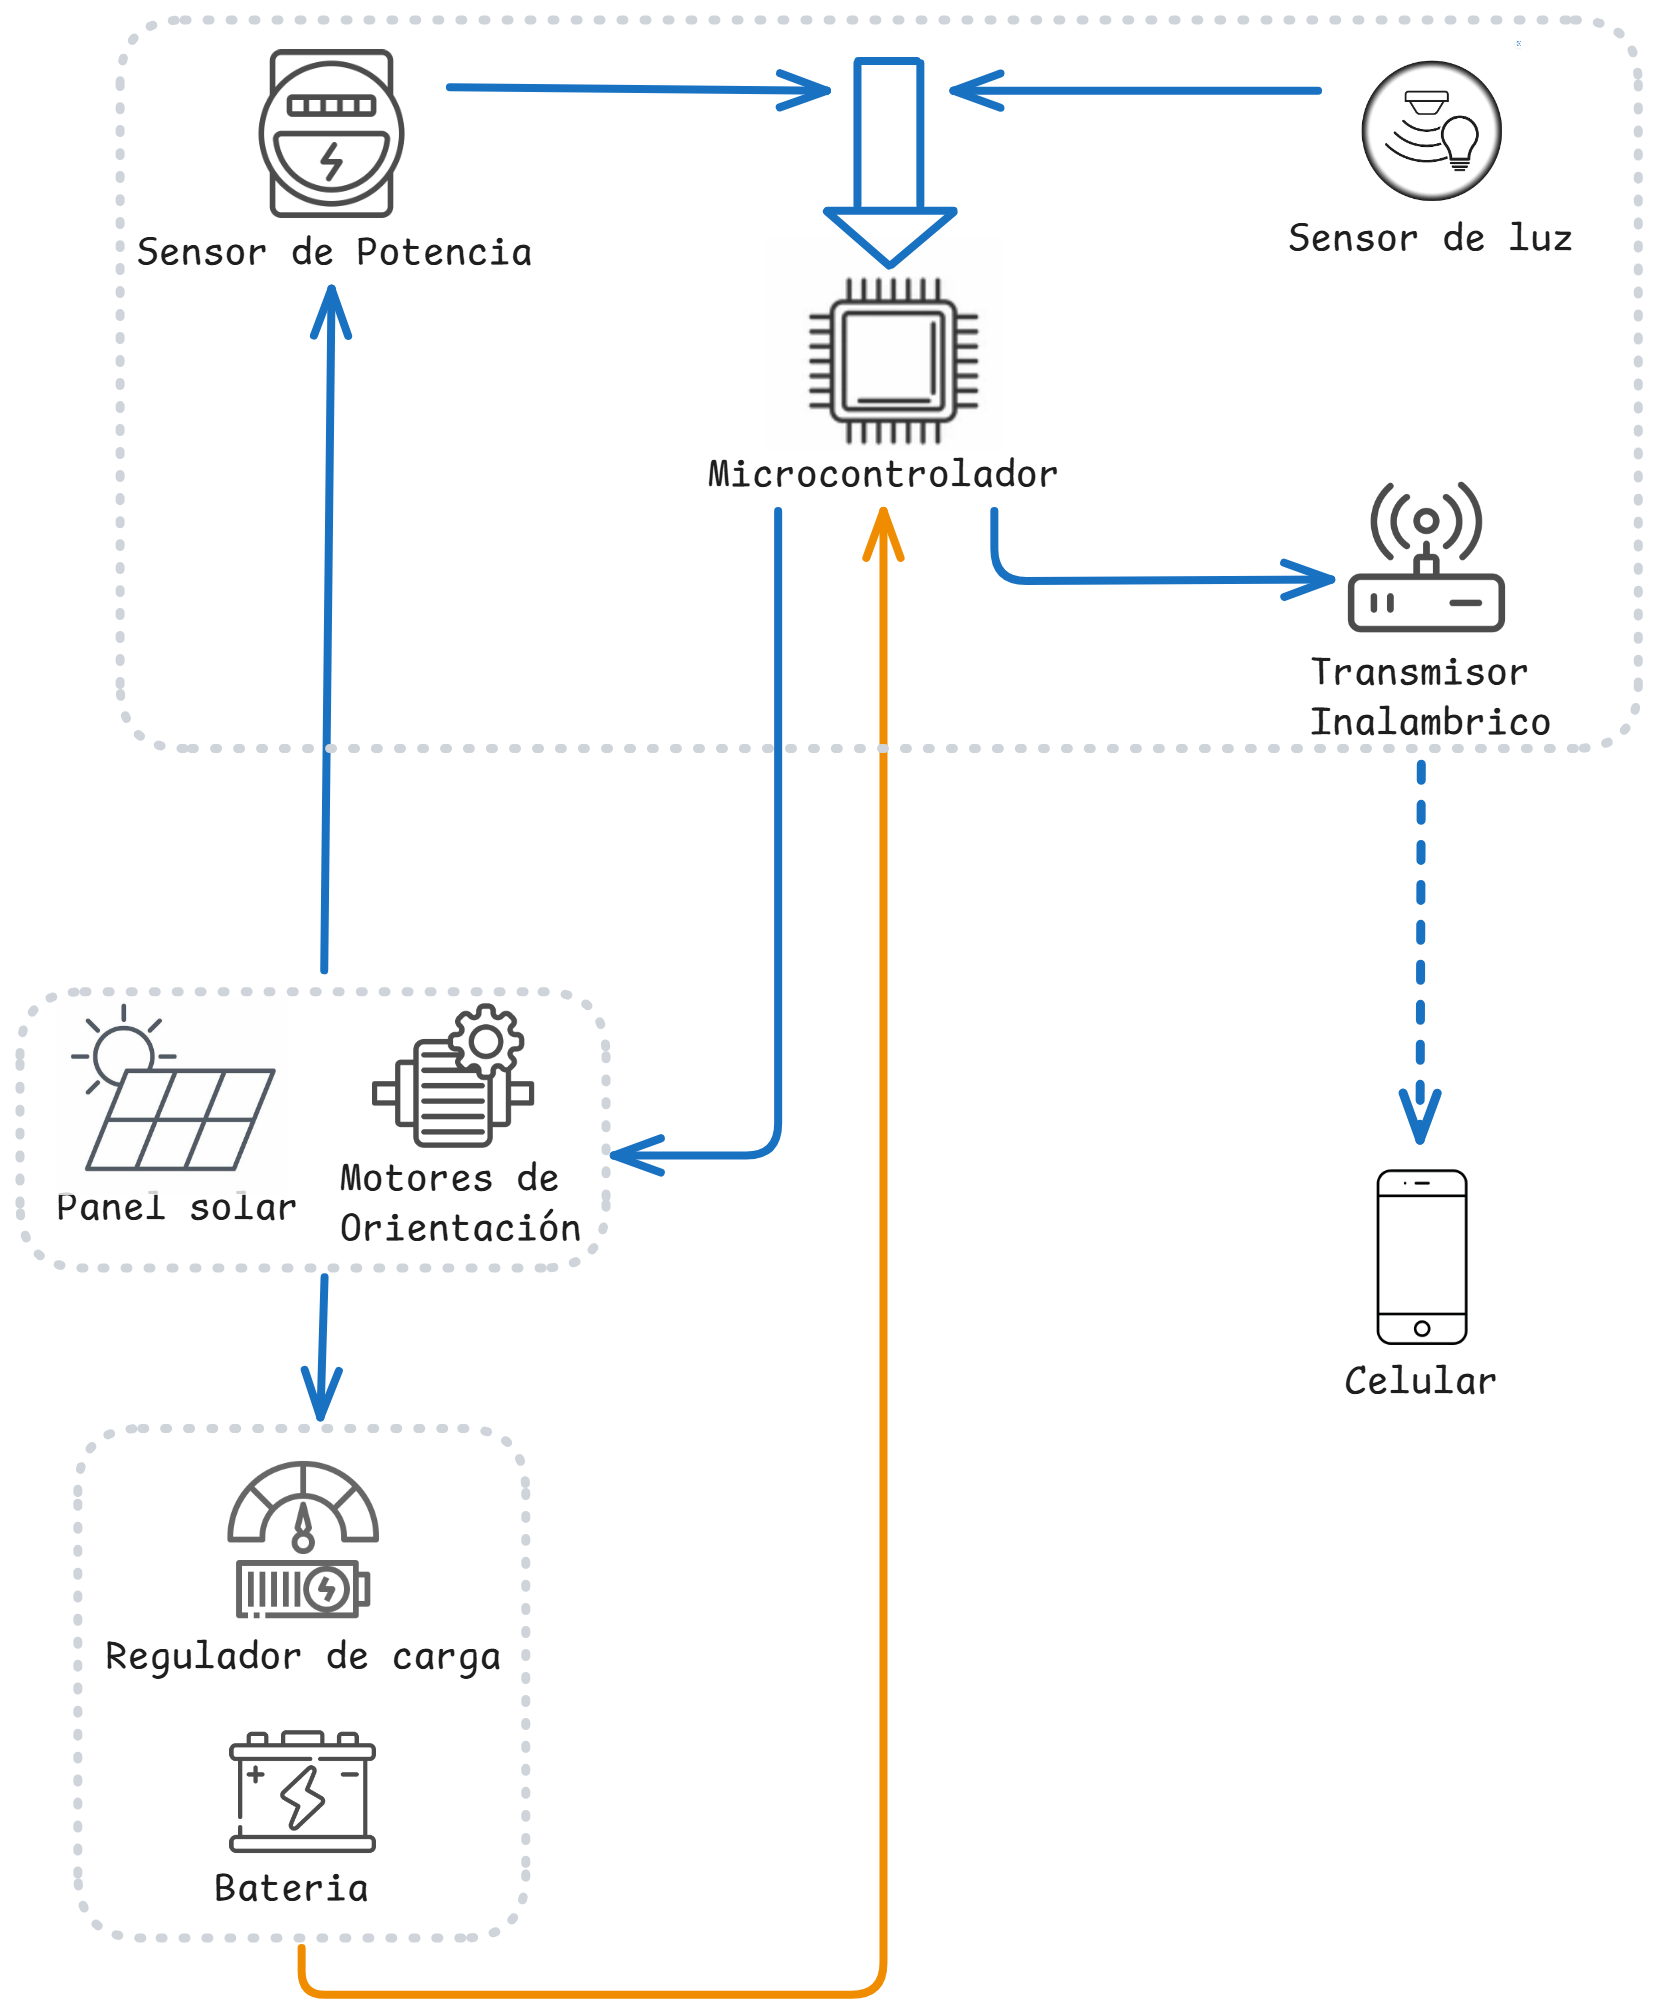
\includegraphics[width=0.7\linewidth]{diagrama_proyecto.png}
    \caption{Figura ilustrativa}
    \label{fig:enter-label}
\end{figure}

%%\hfill{ }\\ {\large \textbf{Objetivos:}}\\

\section{Objetivos}
\subsection{General}

sistema de control de panel solar. Se propone como proyecto la creación de un sistema que rote siguiendo la trayectoria del sol, con el fin de obtener la mayor potencia instantánea posible. Este sistema busca mejorar la eficiencia en comparación con los paneles solares estáticos. Las medidas de potencia, y su horario de medición, van a ser almacenadas y transmitidas para luego ser visualizadas en una interfaz gráfica que incluirá gráficos adicionales y datos históricos de la eficiencia del panel.



\subsection{Particular}
El desarrollo técnico del proyecto abarcaría distintas áreas clave:
\begin{itemize}
        \item Sistema de rotación: la implementación de un mecanismo de rotación de dos ejes para el panel incluido con una base que permita mover al mismo.
        \item Manejo de energía del micro: el sistema debe ser capaz de suministrar energía al microcontrolador desde la batería y el sistema de carga.
        \item Circuito de medición de potencia: debe ser capaz de medir la potencia instantánea usando medidas de tensión y corriente.
        \item Desarrollo de comunicación entre dispositivos: comunicación inalámbrica de datos medidos entre la interfaz gráfica y el microcontrolador.
        \item Creación de interfaz gráfica para móvil: interfaz facil de interpreta, intuitiva y accesible.
        \item Programación de sistema de control: sistema eficiente de rotación y dirección para el movimiento de los motores.
        \item Alimentación del sistema: capacidad de alimentar al sistema con la energía necesaria para su funcionamiento nominal. Se deben considerar las protecciones del sistemas de carga, panel y batería.
\end{itemize}

\section{Especificaciones}
\subsection{Funcionales}
  la gestión energética del microcontrolador, el diseño de un circuito de medición de potencia, el desarrollo de la comunicación entre dispositivos, y la creación de una aplicación móvil que funcione como interfaz gráfica. Para el correcto funcionamiento del mecanismo de rotación, se programaría el sistema de control encargado de ejecutar los ajustes de orientación del panel. Se integraría una fuente de alimentación con batería capaz de garantizar la autosuficiencia energética del dispositivo, permitiendo que la energía excedente sea almacenada.
\subsection{No funcionales}
El sistema deberá ser lo suficientemente robusto como para mantenerse funcional durante períodos prolongados sin intervención externa. La interfaz gráfica sería desarrollada con una lógica de uso simple y accesible, permitiendo su uso por operarios sin conocimientos técnicos avanzados. A su vez, el prototipo serviría como base para eventuales escalados o mejoras futuras, estableciendo un diseño replicable y con potencial de crecimiento.\\
Se plantea que el proyecto sea realizado en un periodo estimado de cinco meses. El proyecto se irá desarrollando en etapas de duración predeterminada, siguiendo un cronograma tentativo inicial.\\

\section{Alcance}
El alcance del proyecto comprendería el diseño, construcción y validación de un prototipo funcional, incluyendo tanto el desarrollo del hardware como del software. No se contemplaría la fabricación a escala ni la comercialización del sistema, ya que esta etapa estaría centrada en demostrar la viabilidad del concepto mediante una unidad operativa.\\

\section{Entregables}
Al finalizar el desarrollo, se entregarían los siguientes productos: el prototipo ensamblado y en funcionamiento, el código fuente del microcontrolador, la aplicación móvil y una guía básica de uso.
Se considerará exitoso si el prototipo logra seguir la trayectoria solar de forma autónoma durante un período prolongado, logra transmitir los datos a la aplicación sin errores y puede operar de forma autosuficiente bajo condiciones de uso normal.\\

\section{Presupuesto}
Finalmente, se estimaría un presupuesto de insumos aproximado de \$150.000, contemplando el costo de sensores, microcontroladores, módulos de comunicación, componentes electrónicos, materiales de construcción y demás insumos necesarios. Esta estimación incluiría un margen de flexibilidad para cubrir ajustes y eventuales imprevistos que pudieran surgir durante el desarrollo del proyecto.\\

\begin{table}[h!]
        \centering
        \begin{tabular}{|l|c|}
            \hline
            Concepto  & Costo Estimado \\ 
            \hline
            Sensores & \$20.000 \\
            Panel solar  & \$23.000 \\
            Motores  & \$25.000 \\
            Soporte pivote & \$8.000 \\
            Microcontrolador  & \$10.000 \\
            Sistema de comunicación  & \$12.000 \\
            Sistema de Alimentación  & \$50.000 \\
            \hline
            \textbf{Total Estimado} & \$148.000 \\
            \hline
        \end{tabular}
        \captionof{figure}{Tabla con precios aproximados consultados al momento de realizar el informe }
        \label{tabla}
        \end{table}

\newpage
\begin{landscape}
    \thispagestyle{empty} % quita número de página si molesta
    \begin{center}
        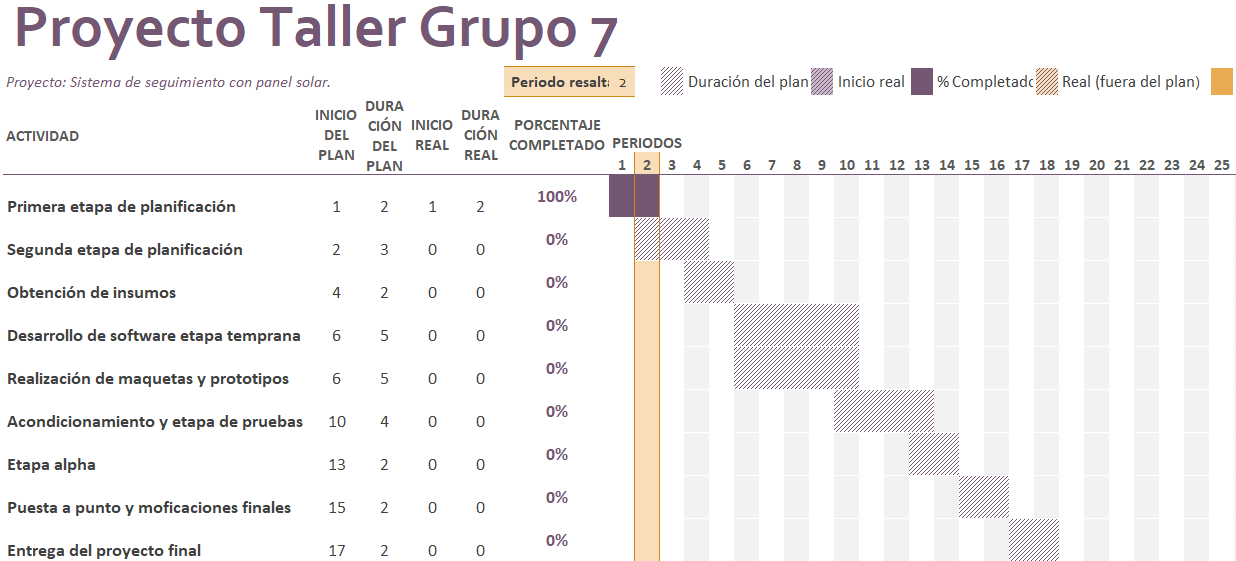
\includegraphics[width=0.95\linewidth]{grantt-V3.png}
        \captionof{figure}{Cronograma en semanas}
        \label{cronograma}
    \end{center}
\end{landscape}
\end{document}
